% questions.tex —— 2011 年·山东卷·文科 · 题目内容片段（无答案）
% 由 tools/generate_projects.py 依来源总账自 2011/2011_数学真题_山东文_试题.md 生成，勿手改（改源 MD 后重跑）


\gkpart{数学}

\begin{gktip}
\textbf{来源说明}：本题面依据固定源 PDF 两页 A3 题面逐栏转录，原卷印刷页码 691–692。固定源不附答案；原页各题与各节均未印分值，记「原页未标」，不补。答案和解析均由本库独立复算。

\textbf{转录说明}：第 18 题第（2）问「并求选出的 2 名教师」的「2」印在第一栏右端（PDF 坐标 $x\approx399\,\mathrm{pt}$，略超出栏宽 $397\,\mathrm{pt}$），按栏裁切取文字层会漏掉它，本库按 600 dpi 原页图补回；这属于取字工具的边界效应，不是原页缺陷。第 19 题第（2）问的「$\parallel$」在原页用斜线符号排印，PDF 文字层不含该符号，同样按 600 dpi 原页图转录。第 11 题原页把「正（主）视图」「俯视图」两个小图印在三个命题之后、四个选项之前，本库按题库体例把图移到四个选项之后，图的内容与标号照原页。第 10 题的（D）在原页是手绘干扰曲线，不是解析函数的图象，本库照原页形状重绘，解析按可辨认特征排除。

\textbf{图形说明}：第 10 题四个选项的函数图象、第 11 题的两个矩形、第 14 题的程序框图、第 19 题的四棱台、第 21 题的容器、第 22 题的椭圆与直线 $l$ 均重绘为 TikZ 矢量图，依原页拓扑重绘，不按比例。原页其余各题无图。
\end{gktip}

\gkpart{一、选择题}

\begin{question}
\gkti{1}设集合 $M=\{x\mid (x+3)(x-2)<0\}$，$N=\{x\mid 1\leqslant x\leqslant 3\}$，则 $M\cap N=$\mbox{（　　）}

（A）$[1,2)$

（B）$[1,2]$

（C）$(2,3]$

（D）$[2,3]$

\end{question}
\begin{question}
\gkti{2}复数 $z=\dfrac{2-\mathrm i}{2+\mathrm i}$（$\mathrm i$ 为虚数单位）在复平面内对应的点所在的象限为\mbox{（　　）}

（A）第一象限

（B）第二象限

（C）第三象限

（D）第四象限

\end{question}
\begin{question}
\gkti{3}若点 $(a,9)$ 在函数 $y=3^x$ 的图象上，则 $\tan\dfrac{a\pi}{6}$ 的值为\mbox{（　　）}

（A）$0$

（B）$\frac{\sqrt3}{3}$

（C）$1$

（D）$\sqrt3$

\end{question}
\begin{question}
\gkti{4}曲线 $y=x^3+11$ 在点 $P(1,12)$ 处的切线与 $y$ 轴交点的纵坐标是\mbox{（　　）}

（A）$-9$

（B）$-3$

（C）$9$

（D）$15$

\end{question}
\begin{question}
\gkti{5}已知 $a$，$b$，$c\in\mathbf R$，命题“若 $a+b+c=3$，则 $a^2+b^2+c^2\geqslant 3$”的否命题是\mbox{（　　）}

（A）若 $a+b+c\neq 3$，则 $a^2+b^2+c^2<3$

（B）若 $a+b+c=3$，则 $a^2+b^2+c^2<3$

（C）若 $a+b+c\neq 3$，则 $a^2+b^2+c^2\geqslant 3$

（D）若 $a^2+b^2+c^2\geqslant 3$，则 $a+b+c=3$

\end{question}
\begin{question}
\gkti{6}若函数 $f(x)=\sin\omega x$（$\omega>0$）在区间 $\left[0,\dfrac{\pi}{3}\right]$ 上单调递增，在区间 $\left[\dfrac{\pi}{3},\dfrac{\pi}{2}\right]$ 上单调递减，则 $\omega=$\mbox{（　　）}

（A）$\frac23$

（B）$\frac32$

（C）$2$

（D）$3$

\end{question}
\begin{question}
\gkti{7}设变量 $x$，$y$ 满足约束条件
\nopagebreak[4]
\[
\begin{cases}
x+2y-5\leqslant 0,\\
x-y-2\leqslant 0,\\
x\geqslant 0,
\end{cases}
\]
则目标函数 $z=2x+3y+1$ 的最大值为\mbox{（　　）}

（A）$11$

（B）$10$

（C）$9$

（D）$8.5$

\end{question}
\begin{question}
\gkti{8}某产品的广告费用 $x$ 与销售额 $y$ 的统计数据如下表：

\begin{center}
\begin{tabular}{lrrrr}
\toprule
广告费用 $x$（万元） & $4$ & $2$ & $3$ & $5$ \\
\midrule
销售额 $y$（万元） & $49$ & $26$ & $39$ & $54$ \\
\bottomrule
\end{tabular}
\end{center}

根据上表可得回归方程 $\hat y=\hat bx+\hat a$ 中的 $\hat b$ 为 $9.4$，据此模型预报广告费用为 $6$ 万元时销售额为\mbox{（　　）}

（A）$63.6$ 万元

（B）$65.5$ 万元

（C）$67.7$ 万元

（D）$72.0$ 万元

\end{question}
\begin{question}
\gkti{9}设 $M(x_0,y_0)$ 为抛物线 $C:x^2=8y$ 上一点，$F$ 为抛物线 $C$ 的焦点，以 $F$ 为圆心、$|FM|$ 为半径的圆和抛物线 $C$ 的准线相交，则 $y_0$ 的取值范围是\mbox{（　　）}

（A）$(0,2)$

（B）$[0,2]$

（C）$(2,+\infty)$

（D）$[2,+\infty)$

\Needspace{0.4\textheight}
\end{question}
\begin{question}
\gkti{10}函数 $y=\dfrac x2-2\sin x$ 的图象大致是\mbox{（　　）}

（A）图 A

（B）图 B

（C）图 C

（D）图 D
\nopagebreak[4]
\begin{center}% 2011 年山东卷文科第 10 题：四个选项的函数图象（选项图）。
% 来源 PDF：普通高考/2011/2011山东文.pdf，SHA-256 bf61cf7bb39a3ccfc57735cd2a7ab34387cbfa6bc86a5e7f8246e13292b0e023。
% 原页：第 1 页（A3 三栏）第 2 栏上部，书页码 691。
% 重绘依据：按原页矢量层实测复刻。原点与 2π 刻度相距 35.61pt，故 1 弧度 = 35.61/(2π) = 5.6698pt，
%   下文坐标一律以弧度为单位的无量纲数（4 即 y=4，6.283 即 2π）。
%   四个子图的坐标系同形：x 轴自原点左伸 11.99、右伸 11.36 弧度；y 轴上伸 6.36、下伸 7.00；
%   y 轴在 y=4 处有一个向右的短刻度（长 0.40），x 轴在 x=2π 处有一个向上的短刻度（长 0.40）；
%   文字位置一律取原页字形盒中心（换算成弧度）：y 标签 (-1.13,7.25)、4 标签 (-1.07,3.87)、
%   2π 标签 (6.29,-1.38)、x 标签 (12.05,-0.98)、选项字母 (-14.03,-6.45)；
%   原点 O 的标注位置各图不同且照原页：(A) 在 x 轴上方 (-1.38,1.13)，
%   (B)(C)(D) 都在 x 轴下方约 (-1.37,-1.45)。
%   原页四图都无网格、无虚线。
%   曲线由原页矢量路径数字化反解：(C) 是 y=x/2-2sin x（残差 0.008），即本题正确图象；
%   (A) 是 y=x/2-2cos x（残差 0.0014），在 y 轴上的截距为 -2；
%   (B) 是 y=x-3sin x（残差 0.002），原页只画在 |x|≤4 内；
%   (D) 是原页手绘的干扰曲线，不是解析函数：每侧三段三次贝塞尔，两支关于原点中心对称，
%   振幅随 |x| 增大（x=±1.56 处约 ∓2.14，x=±7 处约 ±4.5），零点在 0、±3.42、±8.8；
%   本图直接使用原页控制点（原页坐标除以 5.6698pt），拓扑与形状照原页。
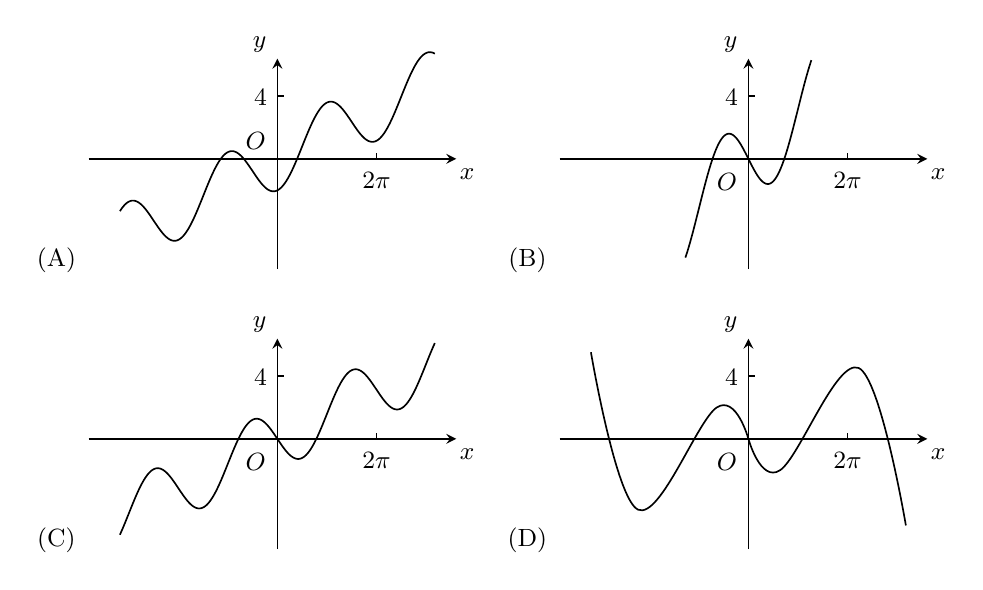
\begin{tikzpicture}[scale=0.20, >=stealth, semithick, font=\small]

  % ===== 四个子图共用的坐标轴（坐标值即原页实测的弧度数；O 的标注各图另放） =====
  \def\axes{
    \draw[->] (-11.99,0) -- (11.36,0);
    \draw[->] (0,-7.00) -- (0,6.36);
    \draw (0,4) -- (0.40,4);
    \draw (6.283,0) -- (6.283,0.40);
    \node at (-1.07,3.87) {$4$};
    \node at (6.29,-1.38) {$2\pi$};
    \node at (12.05,-0.98) {$x$};
    \node at (-1.13,7.25) {$y$};
  }

  % ================= (A) y = x/2 - 2cos x =================
  \begin{scope}
    \axes
    \node at (-1.38,1.13) {$O$};
    \draw[domain=-10:10, samples=300] plot (\x,{\x/2-2*cos(\x r)});
    \node at (-14.03,-6.45) {(A)};
  \end{scope}

  % ================= (B) y = x - 3sin x =================
  \begin{scope}[shift={(29.91,0)}]
    \axes
    \node at (-1.36,-1.45) {$O$};
    \draw[domain=-4:4, samples=200] plot (\x,{\x-3*sin(\x r)});
    \node at (-14.03,-6.45) {(B)};
  \end{scope}

  % ================= (C) y = x/2 - 2sin x =================
  \begin{scope}[shift={(0,-17.78)}]
    \axes
    \node at (-1.38,-1.45) {$O$};
    \draw[domain=-10:10, samples=300] plot (\x,{\x/2-2*sin(\x r)});
    \node at (-14.03,-6.45) {(C)};
  \end{scope}

  % ====== (D) 原页手绘干扰曲线（贝塞尔控制点照原页矢量层） ======
  \begin{scope}[shift={(29.91,-17.78)}]
    \axes
    \node at (-1.36,-1.45) {$O$};
    % 右支：原点 → (2,-2) → (7,4.5) → (10,-5.5)
    \draw (0,0) .. controls (0,0) and (0.767,-2.793) .. (2.000,-2.000)
                .. controls (3.234,-1.207) and (5.590,5.117) .. (7.000,4.500)
                .. controls (8.408,3.883) and (10.000,-5.500) .. (10.000,-5.500);
    % 左支：与右支关于原点中心对称
    \draw (0,0) .. controls (0,0) and (-0.767,2.793) .. (-2.000,2.000)
                .. controls (-3.234,1.207) and (-5.590,-5.117) .. (-7.000,-4.500)
                .. controls (-8.408,-3.883) and (-10.000,5.500) .. (-10.000,5.500);
    \node at (-14.03,-6.45) {(D)};
  \end{scope}

\end{tikzpicture}
\end{center}
\nopagebreak[4]
\Needspace{0.4\textheight}
\end{question}
\begin{question}
\gkti{11}如图是长和宽分别相等的两个矩形。给定下列三个命题：① 存在三棱柱，其正（主）视图、俯视图如图；② 存在四棱柱，其正（主）视图、俯视图如图；③ 存在圆柱，其正（主）视图、俯视图如图。其中真命题的个数是\mbox{（　　）}

（A）$3$

（B）$2$

（C）$1$

（D）$0$
\nopagebreak[4]
\begin{center}% 2011 年山东卷文科第 11 题：长和宽分别相等的两个矩形（正（主）视图、俯视图）。
% 来源 PDF：普通高考/2011/2011山东文.pdf，SHA-256 bf61cf7bb39a3ccfc57735cd2a7ab34387cbfa6bc86a5e7f8246e13292b0e023。
% 原页：第 1 页（A3 三栏）第 2 栏中部，书页码 691。
% 重绘依据：照原页——上下两个全等矩形轮廓，原页实测均 56.68pt × 28.34pt，上下间距 21.25pt；
%   上矩形正下方标「正（主）视图」，下矩形正下方标「俯视图」。无阴影、无虚线、无箭头。
% 坐标取原页 pt：X = x_页 − 566.71，Y = 425.05 − y_页。
\begin{tikzpicture}[x=0.05cm, y=0.05cm, semithick, font=\small]
  % 正（主）视图
  \draw (0,49.59) rectangle (56.68,77.93);
  \node[below, inner sep=3pt] at (28.34,49.59) {正（主）视图};
  % 俯视图
  \draw (0,0) rectangle (56.68,28.34);
  \node[below, inner sep=3pt] at (28.34,0) {俯视图};
\end{tikzpicture}
\end{center}
\nopagebreak[4]
\end{question}
\begin{question}
\gkti{12}设 $A_1$，$A_2$，$A_3$，$A_4$ 是平面直角坐标系中两两不同的四点，若 $\overrightarrow{A_1A_3}=\lambda\overrightarrow{A_1A_2}$（$\lambda\in\mathbf R$），$\overrightarrow{A_1A_4}=\mu\overrightarrow{A_1A_2}$（$\mu\in\mathbf R$），且 $\dfrac1\lambda+\dfrac1\mu=2$，则称 $A_3$，$A_4$ 调和分割 $A_1$，$A_2$。已知点 $C(c,0)$，$D(d,0)$（$c$，$d\in\mathbf R$）调和分割点 $A(0,0)$，$B(1,0)$，则下面说法正确的是\mbox{（　　）}

（A）$C$ 可能是线段 $AB$ 的中点

（B）$D$ 可能是线段 $AB$ 的中点

（C）$C$，$D$ 可能同时在线段 $AB$ 上

（D）$C$，$D$ 不可能同时在线段 $AB$ 的延长线上

\end{question}
\gkpart{二、填空题}

\begin{question}
\gkti{13}某高校甲、乙、丙、丁四个专业分别有 $150$、$150$、$400$、$300$ 名学生，为了解学生的就业倾向，用分层抽样的方法从该校这四个专业共抽取 $40$ 名学生进行调查，应在丙专业抽取的学生人数为\gkblank{}。

\Needspace{0.4\textheight}
\end{question}
\begin{question}
\gkti{14}执行如图所示的程序框图，输入 $l=2$，$m=3$，$n=5$，则输出的 $y$ 的值是\gkblank{}。
\nopagebreak[4]
\begin{center}% 2011 年山东卷文科第 14 题：程序框图。
% 来源 PDF：普通高考/2011/2011山东文.pdf，SHA-256 bf61cf7bb39a3ccfc57735cd2a7ab34387cbfa6bc86a5e7f8246e13292b0e023。
% 原页：第 1 页（A3 三栏）第 3 栏上部，书页码 691。
% 重绘依据：按原页矢量层逐框实测复刻。坐标取原页 pt：X = x_页 − 957.56，Y = 302.20 − y_页。
%   8 个框：开始/结束为圆角矩形 27.98×16.83、27.98×17.00（圆角半径 3.98）；
%   输入、输出为平行四边形（上下边水平、左右边同向斜，横向偏移 6.23，高 17.13）；
%   两个判断为菱形（半对角线 64.32×16.02 与 42.63×10.59）；
%   三个语句框为矩形：y=105 为 42.25×15.80，y=70l+21m+15n 为 102.52×16.33，y=y−105 为 60.61×15.80。
%   连线：主干 6 段竖直，另有 4 段折线——「是」支出菱形左顶点左行 22.63 后下行进 y=105 框；
%   y=105 框底下行 63.30 再右行汇入主干（在菱形 2 与输出之间）；「是」支出菱形右顶点右行 53.50
%   后上行进 y=y−105 框；该框顶上行 5.87 再左行汇入主干（在菱形 2 之上）。全图无虚线、无圆点。
\begin{tikzpicture}[x=0.035cm, y=0.035cm, >=stealth, semithick, font=\small,
  every node/.style={inner sep=1.5pt}]

  % ===== 8 个框 =====
  \draw[rounded corners=3.98] (-13.99,228.40) rectangle (13.99,245.23);                    % 开始
  \draw (-58.82,196.69) -- (-52.59,213.82) -- (58.80,213.82) -- (52.56,196.69) -- cycle;     % 输入
  \draw (0,182.04) -- (64.32,166.02) -- (0,150.00) -- (-64.32,166.02) -- cycle;              % 菱形 1
  \draw (-108.08,119.29) rectangle (-65.83,135.09);                                          % y=105
  \draw (-51.26,119.03) rectangle (51.26,135.36);                                            % y=70l+21m+15n
  \draw (0,84.54) -- (42.63,73.95) -- (0,63.36) -- (-42.63,73.95) -- cycle;                  % 菱形 2
  \draw (65.82,88.66) rectangle (126.43,104.46);                                             % y=y-105
  \draw (-24.74,31.57) -- (-18.51,48.70) -- (24.73,48.70) -- (18.50,31.57) -- cycle;         % 输出
  \draw[rounded corners=3.98] (-13.99,0) rectangle (13.99,17.00);                            % 结束

  % ===== 主干（竖直） =====
  \draw[->] (0,228.40) -- (0,213.82);            % 开始 → 输入
  \draw[->] (0,196.69) -- (0,182.04);            % 输入 → 菱形 1
  \draw[->] (0,150.00) -- (0,135.36);            % 菱形 1（否）→ y=70l+21m+15n
  \draw[->] (0,119.03) -- (0,84.54);             % y=70l+21m+15n → 菱形 2
  \draw[->] (0,63.36) -- (0,48.70);              % 菱形 2（否）→ 输出
  \draw[->] (0,31.57) -- (0,17.00);              % 输出 → 结束

  % ===== 「是」支与回流折线 =====
  \draw[->] (-64.32,166.02) -- (-86.95,166.02) -- (-86.95,135.09);   % 是 → y=105
  \draw[->] (-86.95,119.29) -- (-86.95,55.99) -- (0,55.99);          % y=105 → 主干（输出前）
  \draw[->] (42.63,73.95) -- (96.13,73.95) -- (96.13,88.66);         % 是 → y=y-105
  \draw[->] (96.13,104.46) -- (96.13,110.33) -- (0,110.33);          % y=y-105 → 主干（菱形 2 前）

  % ===== 框内文字 =====
  \node at (0.34,236.85) {开始};
  \node at (0.3,205.75) {输入非负整数 $l$，$m$，$n$};
  \node at (0,165.60) {$l^2+m^2+n^2=0$};
  \node at (-86.61,127.50) {$y=105$};
  \node at (0.34,127.40) {$y=70l+21m+15n$};
  \node at (0.39,74.25) {$y>105$};
  \node at (96.54,96.85) {$y=y-105$};
  \node at (0.19,40.60) {输出 $y$};
  \node at (0.34,9.15) {结束};

  % ===== 分支标签 =====
  \node at (-70.5,175.2) {是};
  \node at (9.3,143.4) {否};
  \node at (43.3,83.2) {是};
  \node at (9.3,56.7) {否};

\end{tikzpicture}
\end{center}
\nopagebreak[4]
\end{question}
\begin{question}
\gkti{15}已知双曲线 $\dfrac{x^2}{a^2}-\dfrac{y^2}{b^2}=1$（$a>0$，$b>0$）和椭圆 $\dfrac{x^2}{16}+\dfrac{y^2}{9}=1$ 有相同的焦点，且双曲线的离心率是椭圆离心率的两倍，则双曲线的方程为\gkblank{}。

\end{question}
\begin{question}
\gkti{16}已知函数 $f(x)=\log_a x+x-b$（$a>0$，且 $a\neq 1$）。当 $2<a<3<b<4$ 时，函数 $f(x)$ 的零点 $x_0\in(n,n+1)$，$n\in\mathbf N^*$，则 $n=$\gkblank{}。

\end{question}
\gkpart{三、解答题}

\begin{question}
\gkti{17}在 $\triangle ABC$ 中，内角 $A$，$B$，$C$ 的对边分别为 $a$，$b$，$c$，已知 $\dfrac{\cos A-2\cos C}{\cos B}=\dfrac{2c-a}{b}$。

（1） 求 $\dfrac{\sin C}{\sin A}$ 的值；

（2） 若 $\cos B=\dfrac14$，$\triangle ABC$ 的周长为 $5$，求 $b$ 的长。

\end{question}
\begin{question}
\gkti{18}甲、乙两校各有 $3$ 名教师报名支教，其中甲校 $2$ 男 $1$ 女，乙校 $1$ 男 $2$ 女。

（1） 若从甲校和乙校报名的教师中各任选 $1$ 名，写出所有可能的结果，并求选出的 $2$ 名教师性别相同的概率；

（2） 若从报名的 $6$ 名教师中任选 $2$ 名，写出所有可能的结果，并求选出的 $2$ 名教师来自同一学校的概率。

\Needspace{0.4\textheight}
\end{question}
\begin{question}
\gkti{19}如图，在四棱台 $ABCD-A_1B_1C_1D_1$ 中，$D_1D\perp$ 平面 $ABCD$，底面 $ABCD$ 是平行四边形，$AB=2AD$，$AD=A_1B_1$，$\angle BAD=60^\circ$。

（1） 证明：$AA_1\perp BD$；

（2） 证明：$CC_1\parallel$ 平面 $A_1BD$。
\nopagebreak[4]
\begin{center}% 2011 年山东卷文科第 19 题：四棱台 ABCD-A1B1C1D1。
% 来源 PDF：普通高考/2011/2011山东文.pdf，SHA-256 bf61cf7bb39a3ccfc57735cd2a7ab34387cbfa6bc86a5e7f8246e13292b0e023。
% 原页：第 2 页（A3 三栏）第 1 栏下部，书页码 692。
% 重绘依据：按原页矢量层逐棱实测复刻。坐标取原页 pt：X = x_页 − 254.98，Y = 588.50 − y_页。
%   底面 ABCD（下底）：A(0,0)、B(102.01,0)、C(134.66,26.52)、D(32.64,26.52)；
%   上底 A1B1C1D1：A1(13.52,49.98)、B1(71.41,49.98)、C1(90.54,64.78)、D1(32.64,64.78)。
%   实线：AB、BC、CC1、C1D1、D1A1、A1A、A1B1、B1C1、B1B、A1B；
%   虚线：DA、DC、DB、DA1、DD1（D 与三条被遮挡的棱，原页不画顶点圆点、不标直角）。
%   原页 D 处的虚线交点处有一小叉，属虚线交叉，不另画。
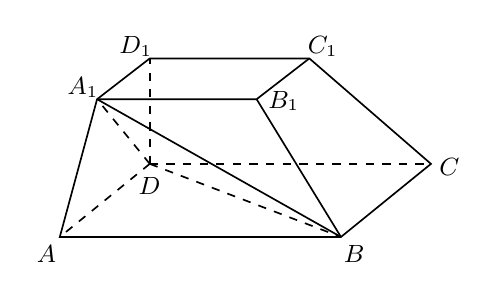
\begin{tikzpicture}[x=0.035cm, y=0.035cm, >=stealth, semithick, font=\small]
  % ===== 顶点 =====
  \coordinate (A)  at (0,0);
  \coordinate (B)  at (102.01,0);
  \coordinate (C)  at (134.66,26.52);
  \coordinate (D)  at (32.64,26.52);
  \coordinate (A1) at (13.52,49.98);
  \coordinate (B1) at (71.41,49.98);
  \coordinate (C1) at (90.54,64.78);
  \coordinate (D1) at (32.64,64.78);

  % ===== 可见的棱（实线） =====
  \draw (A) -- (B) -- (C) -- (C1) -- (D1) -- (A1) -- cycle;
  \draw (A1) -- (B1) -- (C1);
  \draw (B1) -- (B);
  \draw (A1) -- (B);

  % ===== 被遮挡的棱（虚线） =====
  \draw[dashed] (D) -- (A);
  \draw[dashed] (D) -- (C);
  \draw[dashed] (D) -- (B);
  \draw[dashed] (D) -- (A1);
  \draw[dashed] (D) -- (D1);

  % ===== 顶点标记（位置取原页字形盒中心）=====
  \node at (27.57,69.00) {$D_1$};
  \node at (8.42,54.20) {$A_1$};
  \node at (81.27,49.30) {$B_1$};
  \node at (95.37,69.00) {$C_1$};
  \node at (141.37,25.45) {$C$};
  \node at (32.57,18.45) {$D$};
  \node at (-4.83,-6.05) {$A$};
  \node at (106.82,-6.05) {$B$};
\end{tikzpicture}
\end{center}
\nopagebreak[4]
\end{question}
\begin{question}
\gkti{20}等比数列 $\{a_n\}$ 中，$a_1$，$a_2$，$a_3$ 分别是下表第一、二、三行中的某一个数，且 $a_1$，$a_2$，$a_3$ 中的任何两个数不在下表的同一列。

\begin{center}
\begin{tabular}{llll}
\toprule
 & 第一列 & 第二列 & 第三列 \\
\midrule
第一行 & $3$ & $2$ & $10$ \\
第二行 & $6$ & $4$ & $14$ \\
第三行 & $9$ & $8$ & $18$ \\
\bottomrule
\end{tabular}
\end{center}

（1） 求数列 $\{a_n\}$ 的通项公式；

（2） 若数列 $\{b_n\}$ 满足：$b_n=a_n+(-1)^n\ln a_n$，求数列 $\{b_n\}$ 的前 $2n$ 项和 $S_{2n}$。

\Needspace{0.4\textheight}
\end{question}
\begin{question}
\gkti{21}某企业拟建造如图所示的容器（不计厚度，长度单位：米），其中容器的中间为圆柱形，左右两端均为半球形，按照设计要求容器的容积为 $\dfrac{80\pi}{3}$ 立方米，且 $l\geqslant 2r$。假设该容器的建造费用仅与其表面积有关。已知圆柱形部分每平方米建造费用为 $3$ 千元，半球形部分每平方米建造费用为 $c$（$c>3$）千元。设该容器的建造费用为 $y$ 千元。

（1） 写出 $y$ 关于 $r$ 的函数表达式，并求该函数的定义域；

（2） 求该容器的建造费用最小时的 $r$。
\nopagebreak[4]
\begin{center}% 2011 年山东卷文科第 21 题：两端半球、中间圆柱的容器。
% 来源 PDF：普通高考/2011/2011山东文.pdf，SHA-256 bf61cf7bb39a3ccfc57735cd2a7ab34387cbfa6bc86a5e7f8246e13292b0e023。
% 原页：第 2 页（A3 三栏）第 2 栏下部，书页码 692。
% 重绘依据：按原页矢量层实测复刻。坐标取原页 pt：X = x_页 − 605.70，Y = 623.38 − y_页。
%   圆柱段：上下母线 y=56.67 与 y=0，左右两端面在 x=0 与 x=141.68（端面为虚线半椭圆，长半轴 14.17 已被
%   外轮廓遮去一半，只画朝内的一半，照原页）；两个半球各以端面为赤道圆，半径 28.34，圆心在母线中点；
%   半球轮廓为实线椭圆弧（上、下半弧各一），左右对称。
%   虚线：两端面竖直直径（x=0、141.68 处 y=0…56.67），两端面的内侧半椭圆，
%   以及 y=28.34 处的水平点划线（半径 r 的标注线，两端各伸到半球外缘）。
%   标注：l 的双箭头在 y=63.76 处、自 x=3.58 到 138.09；两端的 r 标注各两条（竖直直径上、下半与
%   水平半径），文字位置照原页字形盒中心。原页不画剖面线。
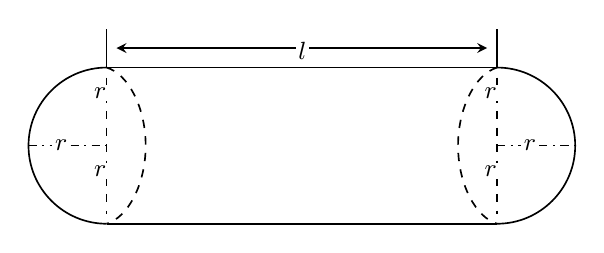
\begin{tikzpicture}[x=0.035cm, y=0.035cm, >=stealth, semithick, font=\small]

  % ===== 半球轮廓（上、下半弧，实线） =====
  \draw (0,56.67) .. controls (-15.60,56.67) and (-28.34,43.94) .. (-28.34,28.34)
        .. controls (-28.34,12.74) and (-15.60,0) .. (0,0);
  \draw (141.68,56.67) .. controls (157.28,56.67) and (170.01,43.94) .. (170.01,28.34)
        .. controls (170.01,12.74) and (157.28,0) .. (141.68,0);

  % ===== 圆柱母线（实线） =====
  \draw (0,56.67) -- (141.68,56.67);
  \draw (0,0) -- (141.68,0);

  % ===== 端面的内侧半椭圆与竖直直径（虚线） =====
  \draw[dashed] (0,56.67) .. controls (7.79,54.36) and (14.17,42.27) .. (14.17,28.34)
        .. controls (14.17,14.41) and (7.79,2.31) .. (0,0);
  \draw[dashed] (141.68,56.67) .. controls (133.89,54.36) and (127.51,42.27) .. (127.51,28.34)
        .. controls (127.51,14.41) and (133.89,2.31) .. (141.68,0);
  \draw[dashed] (0,52.98) -- (0,3.70);
  \draw[dashed] (141.68,52.98) -- (141.68,3.70);

  % ===== 半径标注线（点划线，照原页） =====
  \draw[dash dot] (-28.34,28.34) -- (0,28.34);
  \draw[dash dot] (141.68,28.34) -- (170.01,28.34);

  % ===== l 的双箭头 =====
  \draw[<->] (3.58,63.76) -- (138.09,63.76);
  \draw (0,56.67) -- (0,70.84);
  \draw (141.68,56.67) -- (141.68,70.84);
  \node[fill=white, inner sep=1pt] at (71.00,62.63) {$l$};

  % ===== r 标注（每端三条：竖直半径的上、下两段与朝外的水平半径） =====
  % 原页在标注处把虚线/点划线断开，本图用白底节点遮住线条，效果相同。
  \node[fill=white, inner sep=1pt] at (-2.30,47.38) {$r$};
  \node[fill=white, inner sep=1pt] at (139.38,47.38) {$r$};
  \node[fill=white, inner sep=1pt] at (-2.30,19.08) {$r$};
  \node[fill=white, inner sep=1pt] at (139.38,19.08) {$r$};
  \node[fill=white, inner sep=1pt] at (-16.50,28.58) {$r$};
  \node[fill=white, inner sep=1pt] at (153.58,28.58) {$r$};
\end{tikzpicture}
\end{center}
\nopagebreak[4]
\Needspace{0.4\textheight}
\end{question}
\begin{question}
\gkti{22}在平面直角坐标系 $xOy$ 中，已知椭圆 $C:\dfrac{x^2}{3}+y^2=1$。如图所示，斜率为 $k$（$k>0$）且不过原点的直线 $l$ 交椭圆 $C$ 于 $A$，$B$ 两点，线段 $AB$ 的中点为 $E$，射线 $OE$ 交椭圆 $C$ 于点 $G$，交直线 $x=-3$ 于点 $D(-3,m)$。

（1） 求 $m^2+k^2$ 的最小值；

（2） 若 $|OG|^2=|OD|\cdot|OE|$，

　　① 求证：直线 $l$ 过定点；

　　② 试问点 $B$，$G$ 能否关于 $x$ 轴对称？若能，求出此时 $\triangle ABG$ 的外接圆方程；若不能，请说明理由。
\nopagebreak[4]
\begin{center}% 2011 年山东卷文科第 22 题：椭圆 C、直线 l、射线 OE 与直线 x = -3。
% 来源 PDF：普通高考/2011/2011山东文.pdf，SHA-256 bf61cf7bb39a3ccfc57735cd2a7ab34387cbfa6bc86a5e7f8246e13292b0e023。
% 原页：第 2 页（A3 三栏）第 3 栏中部，书页码 692。
% 重绘依据：原页矢量层实测定标——椭圆外框 x∈[-49.08,49.08]pt、y∈[-28.34,28.34]pt，
%   半长轴∶半短轴 = 49.08∶28.34 ≈ √3∶1，与题设 x²/3+y²=1 完全一致，故取 28.34pt = 1 单位；
%   竖直直线 x=-3 在原页实测位于 -85.01pt = -3 单位，印证该定标。
%   原页要素（单位坐标）：x 轴自 -3.50 到 2.17，y 轴自 -2.00 到 2.27；
%   直线 x=-3 自 y=2.20 到 -1.80；射线 OE 与直线 l 均画到图形之外，照原页截断。
%   本图按几何自洽重排：取 l:y=0.8x+0.5（k>0、不过原点），与椭圆 x²/3+y²=1 交于
%   A(0.5583,0.9466)、B(-1.3802,-0.6042)，中点 E(-0.4110,0.1712)；
%   射线 OE 的斜率为 -0.4167，交椭圆于 G(-1.4045,0.5852)、交 x=-3 于 D(-3,1.2500)。
%   沿射线自 O 向外的次序为 E、G、D，与原页一致；l 的两端各伸出椭圆之外。
%   标注位置照原页相对格局（D 在竖线右侧上方、G 在 OE 与椭圆交点外上侧、E 在交点下方、
%   A 在右上交点外侧、B 在左下交点外侧、O 在原点右下、-3 在 x 轴下方竖线左侧、l 在右上方）。
%   全图无网格、无辅助虚线。
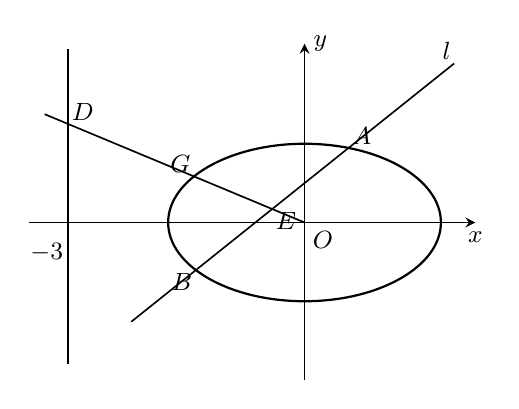
\begin{tikzpicture}[x=1cm, y=1cm, >=stealth, semithick, font=\small]

  % ===== 坐标轴 =====
  \draw[->] (-3.50,0) -- (2.17,0) node[below, inner sep=3pt] {$x$};
  \draw[->] (0,-2.00) -- (0,2.27) node[right, inner sep=3pt] {$y$};

  % ===== 椭圆 =====
  \draw[thick] (0,0) ellipse ({sqrt(3)} and 1);

  % ===== 直线 x = -3 =====
  \draw (-3,2.20) -- (-3,-1.80);

  % ===== 射线 OE（过 O、E、G、D 的直线，画到 D 之外）=====
  \draw (0,0) -- (-3.30,1.3751);
  % ===== 直线 l（过 A、B，两端伸出椭圆）=====
  \draw (-2.20,-1.2600) -- (1.90,2.0200);

  % ===== 标注 =====
  \node[above right, inner sep=1pt] at (-3,1.2500) {$D$};
  \node[above left, inner sep=1pt] at (1.90,2.0200) {$l$};
  \node[above left, inner sep=1pt] at (-1.4045,0.5852) {$G$};
  \node[above right, inner sep=1pt] at (0.5583,0.9466) {$A$};
  \node[below right, inner sep=1pt] at (-0.4110,0.1712) {$E$};
  \node[below right, inner sep=1pt] at (0.06,-0.07) {$O$};
  \node[below left, inner sep=1pt] at (-1.3802,-0.6042) {$B$};
  \node[below left, inner sep=1pt] at (-3.02,-0.22) {$-3$};

\end{tikzpicture}
\end{center}
\nopagebreak[4]

\end{question}